%# -*- coding: utf-8-unix -*-
%%==================================================
%% chapter01.tex for SJTU Master Thesis
%%==================================================

%\bibliographystyle{sjtu2}%[此处用于每章都生产参考文献]
\chapter{Introduction}
\label{chap:intro}
\section{Motivation and Contribution}
In many real world applications, data is collected incrementally. For example, the large-scale image classification dataset ImageNet is becoming larger and larger when more notations become available. For vision-based applications like assisted ambient living, intelligent car driver assistants, robotic arms in logistics center and autonomous supermarkets, they share the need to distinguish between different categories. More importantly, they also share the need to update their knowledge over time, by updating their models to recognize new unseen categories whenever new categories become available. Let us take the main origination of this project as an example. Imagine a commercial system that can classify merchandise correctly based on the image of the merchandise, as illustrated in Fig.~\ref{fig:merchandise}. It has a large potential to be used by automatic robotic arms used in automatic logistics center or autonomous supermarkets. A robotic arm is shown in Fig.~\ref{fig:arm}. Since there will always be new types of merchandise emerging, this system should always adapt to new merchandise types but also not forgetting the learned merchandise types. It can be summarized as follows: Suppose you already have a image classifier that can classify $N$ classes. Then when a new type of merchandise came, using the new training data, you will have to extend its knowledge to classify $N+1$ classes, without needing to re-train everything from scratch, which will cost much time and energy.

\begin{figure}[!htp]
	\centering
	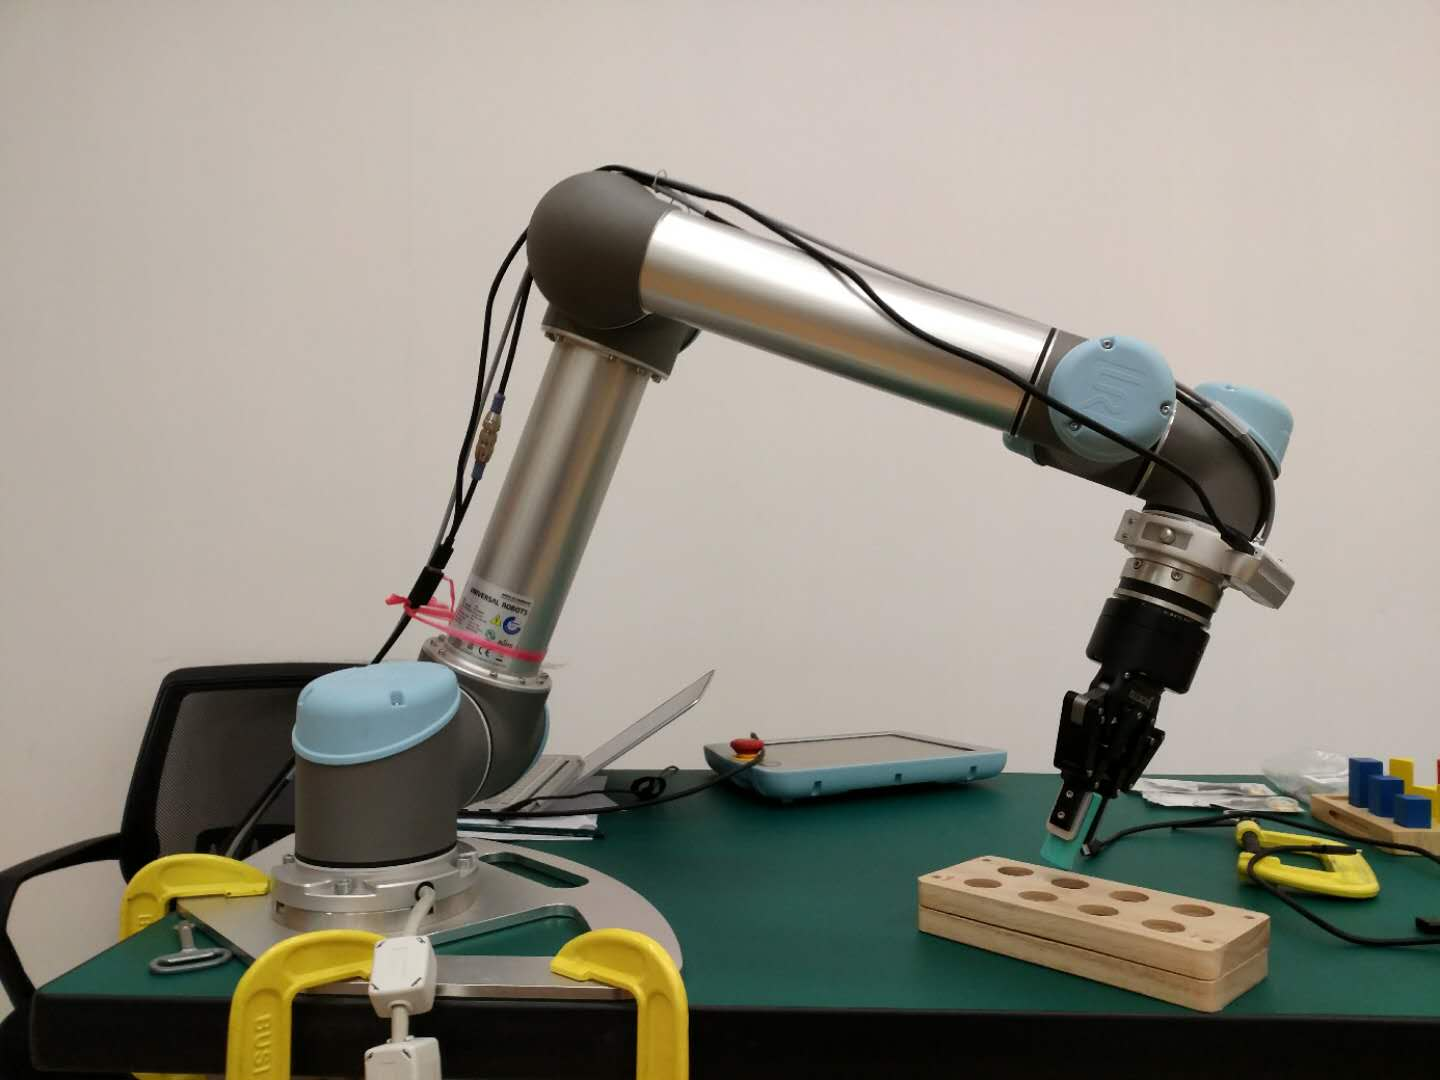
\includegraphics[width=12cm]{arm.jpg}
	\bicaption[Example of a robotic arm for autonomous logistics center]
	{可用于物流系统的机械臂示意图}
	{Example of a robotic arm for autonomous logistics center}
	\label{fig:arm}
\end{figure}
\begin{figure}[!htp]
	\centering
	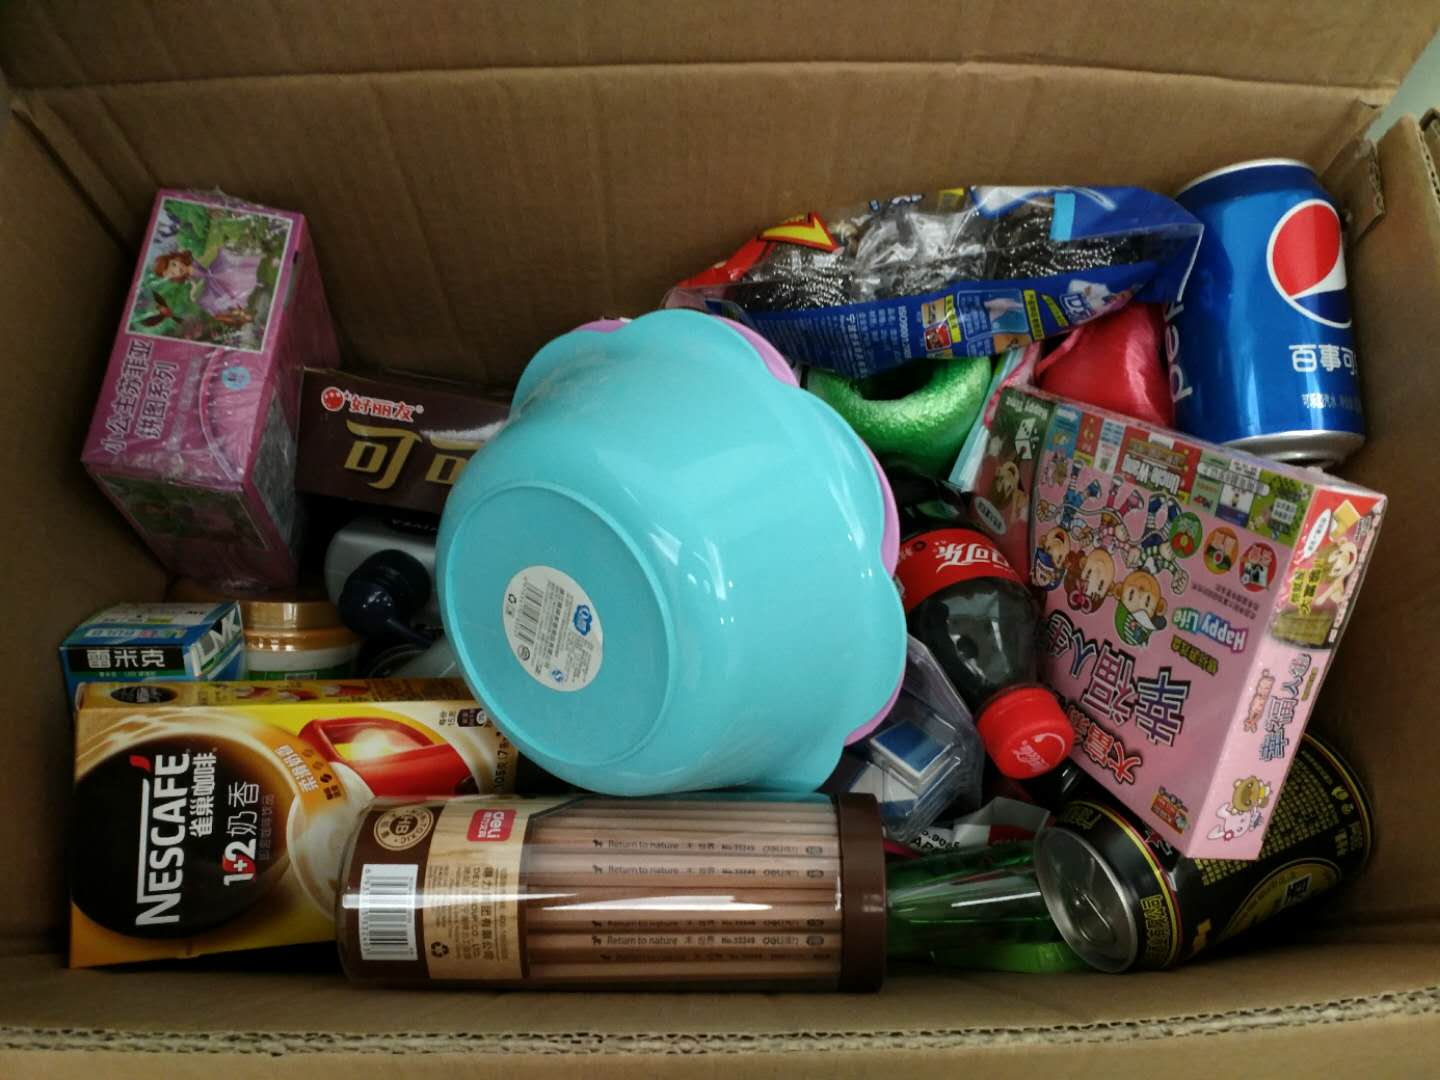
\includegraphics[width=12cm]{merchandise.jpg}
	\bicaption[Example of various types of merchandise]
	{不同类别的商品示意图}
	{Example of various types of merchandise}
	\label{fig:merchandise}
\end{figure}

In recent years, deep learning, or to be more concrete, deep convolutional neural network(CNN), is the main method on these computer vision problems. Shown in the examples, it is essential that we had methods that can accommodate the newly increased data quickly based on the previous deep learning model, without having to train the whole model with the entire data from scratch. The reasons are obvious. Training the whole deep learning model from scratch would be too time-consuming and energy-consuming. For example, training a image classification model for ImageNet-1k Dataset\cite{deng2009imagenet} using $32\times4d$ ResNeXt-101\cite{xie2017aggregated} model takes 5 days on 8 GPUS. If we retrain the entire model every time new classes of data or more data from the same class become available, the expense will be enormous. This is even worse in commercial scenarios: imagine several new types of merchandise arrive every day, if we retrain the model from scratch, merchandise would have to wait up to several days to be classified and processed, which is unacceptable for real use.
\begin{figure}[!htp]
	\centering
	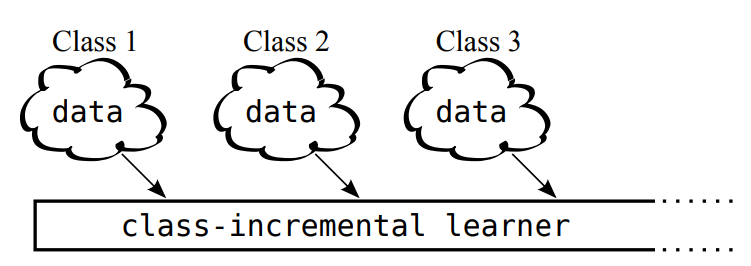
\includegraphics[width=12cm]{classincremental.png}
	\bicaption[Illustration of class-incremental learning]
	{类别增量学习的示意图}
	{Illustration of class-incremental learning}
	\label{fig:classincremental}
\end{figure}
A term that describes this kind of problems in literature is called incremental learning. Unfortunately, few papers considered this type of problem in history. The best methods for now are far from valuable use, and there is no common benchmark or metric in this area. In this paper, we hope to propose methods to this type of learning problems. There are many different terms that are relevant to this topic but might be slightly different in the conditions, including lifelong learning, multitask learning, class-incremental learning, etc.\cite{utgoff1989incremental}, which we will discuss in further detail in related work section.

To match closely with real use, we considered class-incremental learning on image classification problems, illustrated in Fig.~\ref{fig:classincremental}, which means that each time one new class of training data arrive. By combining techiques of hard negative mining, we proposed an algorithm with low computation requirements while achieving relatively good accuracy. We conducted our experiments in image classification problems, using the datasets CIFAR-10 and CIFAR-100\cite{krizhevsky2009learning}. We used ResNet\cite{he2016deep} and DenseNet\cite{huang2017densely} as representative deep learning models and showed similar trends, which reveals our method is generic for deep learning models. We proposed and compared between various methods, and showed that we can indeed achieve similar high performance within $5\%$ of the total training time for a model retrain, by using a strong baseline method. Furthermore, we show our algorithm can control the trade off between training time and accuracy by adjusting a hyper-parameter.

We also noted that incremental learning for deep neural networks is a fundamental and tough problem and this field is relatively premature. There are not many existing works or common benchmark, and our method is still not satisfying for commercial use. We hope more research could be conducted in incremental learning for deep neural networks in the future.
\section{Related work}
\subsection{Deep Learning in Computer Vision}
The first successful use of deep learning comes from image classification area. Since the success of AlexNet\cite{krizhevsky2012imagenet} in 2012, deep learning has developed in a tremendous pace. The performance of image classfication as well as other applications of deep learning improve fast as newer and better model architectures are proposed.

After AlexNet, VGGNet\cite{simonyan2014very} was proposed that used up to more than 30 layers of neural network and significantly improved the performance. At the same time, Google developed a series of deep model architectures\cite{szegedy2015going,szegedy2016inception,szegedy2016rethinking} by utilizing multi-path kernels and outperformed VGGNet. In 2015, Kaiming He proposed ResNet\cite{he2016deep}, using a generic methodology to add shortcut connections between layers that became widely used in later networks. He further refined his work in \cite{he2016identity}, allowing successful training of up to 1202 layers, and surpassed the classification accuracy of human eye. Many variations of ResNet also emerged that year, including Wide ResNet, Later, DenseNet\cite{huang2017densely} proposed to use even denser connections than ResNet, linking every previous layer to the current layer, and replacing sum operator with concatenation. ResNeXt\cite{xie2017aggregated} and Xception\cite{chollet2016xception} make use of group convolution to further improve the performance. In 2017, there continued to have innovations in network architecture which boosted the performance, like Dual Path Networks\cite{chen2017dual} which introduced a novel architecture, and Gradually Updated Neural Networks\cite{qiao2017gradually} that rethinked and improved the calculation method of convolutional layers. Worth mentioning, Google also contributed a lot on automatic searching for the network architecture, and they named the product 'AutoML'. Using their algorithm, they have successfully discovered several interesting and effective architectures, like the state-of-the-art automatically discovered networks NASNet-A\cite{zoph2017learning}, PNASNet\cite{liu2017progressive} and AmoebaNet\cite{real2018regularized}.

Besides the stream of designing better model architectures, some techniques or auxiliary layers are also introduced to boost the network's performance. Dropout\cite{srivastava2014dropout} was proposed to prevent overfitting and improve the performance. It is commonly used in small datasets but is rarely used today on ImageNet dataset. Batch Normalization\cite{ioffe2015batch} enabled much easier training of deep neural networks. By adding batch normalization layer after the convolutional layer, we are able to use much simpler weight initialization and optimization algorithms, and are able to successfully train deeper networks even without residual connections\cite{he2016deep}. Squeeze-and-Excite Block\cite{hu2017squeeze} is a simple but effective component to be placed after each stage of a network. It consists of global pooling and fully connected layers, and re-weights the features from the corresponding stage. It adds really low overhead (very few extra parameters compared to the whole network) but is able to effectively boost the network performance.

To the best of the authors knowledge, the top performing network on the most authoritative image classification dataset ImageNet-1K is SENet-154\cite{hu2017squeeze}, which is mainly composed of a ResNeXt network and Squeeze-and-Excite Blocks. It reaches up to $16.88\%$ top-1 error and $3.58\%$ top-5 error on ImageNet-1K dataset.

\subsection{Incremental Learning}
Incremental learning is a term describing the scenario we are considering. By incremental, it either refers to new data or new tasks. Generally speaking, it includes adding new samples from existing classes, new samples from new classes that are previously unseen, new dataset, new tasks, etc. In incremental learning, we hope to reuse the trained network from earlier data or task to minimize the extra computation needed to learn the new task, as well as trying to maintain the performance on old tasks. The worst computation bound and the highest performance bound, would usually be to train the whole network from scratch using all old and new data. Incremental learning tries to learn new data as quick as possible with the least damage of performance to the old data.

Traditionally, many papers proposed solutions to incremental learning based on existing learning models, including decision trees\cite{utgoff1989incremental}, neural networks\cite{polikar2001learn++}, and SVM\cite{diehl2003svm}. They are heavily based on the concrete model itself, and used the concrete properties of the corresponding machine learning model. Therefore, they are offer little guidance to models using deep learning.

\subsubsection{Some early attempts}
In recent years, deep neural networks have enabled much better models with higher accuracy. Accordingly, several relevant papers have proposed solution to incremental learning for deep neural networks. When applied to deep neural networks, there are three straightforward and commonly used strategies that can be applied. The idea is to reuse the parameters that extract the convolutional features from the trained network. Let us assume that a convolutional neural network has a set of parameters $\theta_f$ and $\theta_o$, where $\theta_f$ refers to the parameters for convolution layers (feature extractor) and $\theta_o$ refer to the parameters of the final fully connected layers that do classifying. When new data or task is arrived, we use $\theta_n$ to denote the new final layers for the new data or task. Then the three strategies can be conducted as follows to learn $\theta_n$ while benefitting from the previously learned $\theta_f$.
\begin{itemize}
	\item \textbf{Feature Extraction}: $\theta_f$ and $\theta_o$ are unchanged, and only the new parameters $\theta_n$ are learned. Since $\theta_n$ operates on top of $\theta_f$, we can interpret $\theta_f$ as a fixed feature extractor, and we will use the fixed feature extractor to extract features on new data or task, and learn the new corresponding classifier.
	\item \textbf{Fine-tuning}: $\theta_f$ and $\theta_n$ are trained for the new data. We can duplicate another network that has the parameters $\theta_f$ and $\theta_n$, or simply share the parameters $\theta_f$. We can use a small learning rate to train the new network to prevent the trained parameters $\theta_f$ to drift too much away.
	\item \textbf{Joint Training}: $\theta_f$, $\theta_o$ and $\theta_n$ are further trained together. We can simply train the network using all data available.
\end{itemize}

However, these methods have drawbacks. Feature extraction is only suitable when the feature extractor is already generic enough and the data increments only for a few times. After all, the convolutional parameters might only be in global or local optima for the previously trained data, but it cannot be optimal for all data, including old and new data, because they are not trained using the new data. Thus, the performance tends to degrade if the feature extractor is fixed too early. There are also variations based on this method. For example, \cite{mensink2012metric} utilized the nearest class mean classifier(NCM). NCM represent each category with a prototype vector, which is the average vector feature of all examples so far observed. There is no need to store all training examples, since this vector can be incrementally computed from the stream of data. It classifies a new example by assigning it the category label which has a prototype vector most similar to the feature vector of the example, with regards to a metric that is learned from data. NCM worked well despite its simplicity than prior work, but is still flawed in that it cannot easily be extended to nonlinear data representations.

For fine-tuning, if we share the parameters $\theta_f$, the performance for old data would become very poor, and eventually similar to random guessing, since $\theta_o$ is optimized for the older version of $\theta_f$. This phenomenon is also called catastrophic forgetting or catastrophic interference in literature\cite{goodfellow2013empirical}. The paper by Goodfellow \cite{goodfellow2013empirical} conducted a comprehensive survey on this phenomenon that happened on gradient based deep neural networks. Another option is to duplicate the network for the new data or task. But there will be twice computation load, and we will need to train another extra classifier to distinguish between new and old data to inform the system which model to use, which is not practical. 

Joint training is likely to provide the best performance, given that we care both accuracy for the old data and accuracy for new data. We define the performance upperbound of incremental learning as $P_{upper}$. It is obvious that $P_{upper}$ can be obtained by training the whole network from scratch using all old and new data. The performance of joint training, in many times, can reach the upper bound $P_{upper}$, since all parameters of the network are further trained. However, the drawback is that it can be time consuming and costly.

\subsubsection{Other methods}
Therefore, many other methods are proposed in recent years to remedy this problem. Learning without forgetting\cite{li2017learning} is a famous paper working on sequential multi-task learning without forgetting old tasks.
Utilizing the distillation loss proposed by Hinton\cite{hinton2015distilling}, they proposed to use distillation loss in addition to classification loss for new tasks. In this way, past data for the old task can be completely discarded. It seems to relate closely to incremental learning, especially by the paper name. However, this algorithm cannot fit well for incremental learning for the following reasons. First, in incremental learning, there is only one task in whole, and the only change that might happen to the output of the network is to add additional outputs for new class scores. Hence from beginning to end, only one softmax classifier will be used in incremental learning setting. Then it will be difficult to use both distillation loss and classification loss, because there is only one softmax function. One idea is to still apply the distillation loss on old classes, and train only with data for new classes. This option leads to very poor and unstable performance, because the old data is not used at all. Moreover, the balancing factor $\lambda$ between distillation loss and classification loss is hard to tune. Worse, it is impossible to apply the algorithm when only one new class arrives, then the model would explode because there is always only one correct class: the new class.

Due to the difficult reasons, there are also several papers that tries from a different perspective. They try to evolve the network dynamically when new data or task arrives, like \cite{yoon2017lifelong,rosenfeld2017incremental,sarwar2017incremental,rusu2016progressive}. By evolving the network, they manage to keep the outputs of the original data unchanged or little changed, so that new parameters can be learned for new data, and the accuracy of old data can be maintained by the old parameters. They carefully design the network transformation such that the output for past data remain the same. However, these methods have obvious drawbacks in common. First of all, the network will become extremely large if we continue to add new data. Secondly, to ensure the performance on old data do not deteriorate, the older parameters will remain constant or change little. Then, the old features might be very weak and biased, because they are only trained on a smaller percent of data. Better global features can only be learned by newer parameters. In this case, the network will become very redundant, worsening the network capacity exploding problem.


Perhaps the most relevant and similar paper with us is the paper ICaRL\cite{rebuffi2017icarl}. ICaRL\cite{rebuffi2017icarl} is a recent proposal for class-incremental image classification systems, that maintain only a limited set of exemplars for old data. Their algorithm is designed specially for class-incremental systems, that is, every time one or several new classes of data arrives. This is exactly the same use case with our goal, since we want to learn new types of merchandise every time. We break down their algorithm into three aspects to briefly explain it:
\begin{itemize}
	\item Classification. For classification, they do not adopt the common softmax classifier. Instead, ICaRL relies on sets of exemplar images selected by the algorithm. There is one set for every known class. With the set, it runs every exemplar image through the trained feature extractor (composed of a convolutional neural network), and computes the mean of exemplars for each class set. Finally, they do classification by choosing the nearest prototype by L2-norm.
	\item Training. Each time new data arrives, they train the feature extractor using the previous exemplar sets, and the new samples for the new class. Finally, the exemplar set is updated with a new exemplar set.
	\item Architecture. They use a convolutional neural network, $\varphi=X\to R^d$ to perform feature extraction. Moreover, they normalize the feature vectors and including the results of any operations on the feature vectors.
\end{itemize}
We think ICaRL has several drawbacks, for example, applying the nearest-neighbor approach directly on feature maps does not make much sense, since small objects would yield to smaller average values on feature maps while larger objects are likely to have larger activation values. We show in our experiments that our results outperform ICaRL, with similar training time.

\section{Hard Negative Mining}

Hard negative mining refers to the idea of selectively choosing samples to train, preferably the hard ones that the model is not doing well. This idea was traditionally called dataset bootstrapping in literature\cite{sung1996learning}. Hard negative mining has long been heavily used in object detection research. In 2005, Triggs and Dalal\cite{dalal2005histograms} used it to train SVMs for pedestrian detection. Hard negative mining became most popular in papers in recent years\cite{shrivastava2016training,liu2016ssd,girshick2014rich,girshick2015fast,ren2015faster}. Those papers use this technique to balance the negative background training samples and the positive object region samples. Hard negative mining technique has also been successfully applied to various other learning algorithms, such and boosted decision trees, and shallow neural networks. 

There are two hard negative mining methods commonly use. The first algorithm is used specially when optimizing SVMs. In the algorithm, it maintains a dynamic set of examples and changes between training the SVM to convergence in the dynamic set, and updating the dynamic set by adding some examples and removing some others in a specific way\cite{felzenszwalb2010object}. Under SVM, they assume that an example is easy if that example falls beyond the current SVM model's margin. Conversely, they regard an example as hard if it violate the margin of the current model. Importantly, the dynamic set is a small subset of the whole training set, so that the method can save computation.

The second way is applied for non SVM models. It usually starts with a set of positive examples and a randomly sampled set of negative examples. As the model learns, it gradually prioritize the sampling of harder examples, which means the examples that the model predicts poorly. This kind if method is the method we will refer to in our algorithm. However, it is worth noting that the kind of method is rather empirical and does not have any convergence guarantees. Most people are using this technique because it behaves empirically well, so do us.

In 2017, researchers at Facebook proposed a better algorithm to substitute the hard negative mining step in object detection, using a hand-designed loss function called focal loss\cite{lin2017focal}. This loss function automatically enlarges the loss for harder examples that the model is performing poorly, and minimizes the loss for easier examples. As a result, hard negative mining step is no longer needed because the focal loss function automatically adjusts the weights for different examples. However, the focal loss function is not suitable for the incremental learning problem we are considering here. It is because we wish to use as much old examples as possible to save computation time, which is in contradiction with focal loss detection algorithm that uses all examples in the training set to train.

\chapter{Background}

\section{Image Classification}
\subsection{Overview}
Image classification problem is one of the core problems in computer vision. The task is to assign every image an label from a predefined set of labels. Although it seems simple, it has a large variety of applications. Many other seemingly different computer vision problems such as segmentation and object detection often take heavy use of the techniques and methods in image classification. 

There are many challenges in this kind of problem, some of which are listed below:
\begin{itemize}
	\item Scale variation. An object in an image may vary by scale.
	\item Viewpoint variation. The viewpoint of the camera might be different, but it should not affect the predictions.
	\item Intra-class variation. The same class often has different appearance, for example red balls and green balls both belong to ball category.
	\item Occlusion. Often many parts of an object is occluded, but we should still be able to recognize it.
\end{itemize}
Therefore, image classification models should ignore the irrelevant variations, but capture the general characteristics to differentiate different categories.

Most common approaches nowadays are data-driven. It means that we can obtain a large amount of training data, and we will be able to test our model on a test set, before real use. The common strategy is to train a model using the annotated training set, i.e., supervised learning, and then compare the accuracy on the test set to measure a model's performance. Concretely, this process can be summarized into the following three steps:
\begin{itemize}
	\item \textbf{Input}: The input is a set of annotated training set, consisting of a set of N images and its corresponding annotated label(the label might not be $100\%$ correct but should be mostly correct for the model to work well.).
	\item \textbf{Learning}: This step is called training a classifier, or learning a model. The task is to use the above mentioned training set to learn to differentiate different classes.
	\item \textbf{Evaluation}: In this step, we evaluate our trained model/classifier on a new set of annotated images that the model has never seen before, and see if the predicted categories match the true labels of the images. 
\end{itemize}

\subsection{Score Function and Loss Function}
In this section, I will introduce linear classification method, the most common basic approach used in recent years that forms the basis of the final layer of deep neural networks. This approach has two major components, a score function that maps the raw image or features to class confidence scores, and a loss function that quantifies the degree to which the confidence scores match the ground truth labels. As shown below, it is in fact an optimization problem with respect to the parameters of the score function.

Let us assume that there is a training set $\mathbf{X}$, consisting of $N$ images $x_i \in R^D$, each annotated with a label of its category $y_i$. Here $i = 1 ...N$ and $y_i \in 1 ... K$. This means that the image dimension is $D$ (for example, $D=32\times32\times3$ for a $32\times32$ pixel colored image) and there are $K$ distinct categories. In linear mapping, we would first apply a linear projection to get the class score $f(x_i; W, b)$:
\begin{align}
f(x_i; W, b) = Wx_i + b
\end{align}

With regards to the loss function, it quantifies the degree to which the class scores match the ground truth labels. Intuitively, the loss function would be low or close to zero if our predictions are very accurate, and it would be very high if the model is doing poorly. Thus, as an optimization problem, we would like to minimize the loss function. We would briefly introduce the SVM loss and softmax loss function here. Note that the softmax loss function is the most commonly used in deep neural networks for image classification.

The Multi-class Support Vector Machine loss is such a loss that it wants the correct class for an image to have a score higher than the other classes by a specified margin $\Delta$,illustrated in Fig.~\ref{fig:svm}. For simplicity, we let $s_i = f(x_i; W, b)$. The multi-class SVM loss can be expressed as:
\begin{align}L_i = \sum_{j\neq y_i} max(0, s_j - s_{y_i} + \Delta)\end{align}
It is also called the hinge loss. The total loss would be the sum of the loss from each class $L_i$.
\begin{figure}[!htp]
	\centering
	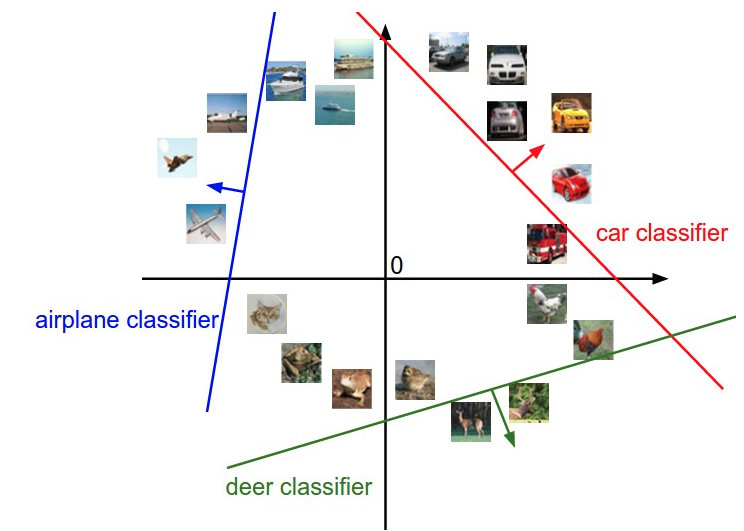
\includegraphics[width=10cm]{svm.png}
	\bicaption[An example of SVM classifier]
	{SVM分类例子例子}
	{An example of SVM classifier}
	\label{fig:svm}
\end{figure}
The softmax loss is a generalization of the binary logistic regression loss to multiple classes. In the softmax loss, we interpret the class scores as the unnormalized log probabilities. Therefore, to obtain the probabilities, we will first exponentiate them and then normalize so that they sum to one: 
\begin{align}
P(Y_i|x_i;W) = \frac{e^{f_{y_i}}}{\sum_j e^{f_j}}
\end{align}, where $f_j$ means the $j$th element of the class scores vector.
In this probabilistic interpretation, we then minimize the negative log likelihood of that correct class, which is like performing Maximum Likelihood Estimation. Thus the softmax loss can be written as:
\begin{align}L_i = -log\left( \frac{e^{f_{y_i}}}{\sum_j e^{f_j}}\right)\end{align}
or its equivalent,
\begin{align} L_i = -f_{y_i} + log \sum_j e^{f_j}\end{align}
It is also called the cross-entropy loss. With the linear score function and the loss function, we are ready to extend them to deep neural networks, which will be introduced briefly in the next section.



\section{Deep Neural Networks}
It is often claimed that the area of Neural Networks was originally inspired by biological neural systems. However, the neural network referred in this paper, and including common literature, is a much simplified mathematical operation, compared to real biological neural networks. A basic unit is illustrated in Fig.~\ref{fig:singleneuron}.
\begin{figure}[!htp]
	\centering
	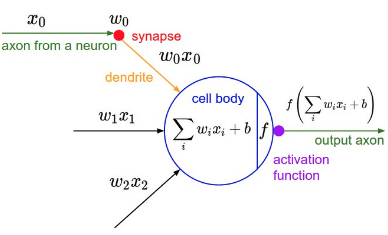
\includegraphics[width=7cm]{singleneuron.png}
	\bicaption[An illustration of a single neuron]
	{单个神经元示意图}
	{An illustration of a single neuron}
	\label{fig:singleneuron}
\end{figure}
Based on the single neuron, we are able to stack many of them to form a multi-layer neural network, as illustrated in Fig.~\ref{fig:nn}.
\begin{figure}[!htp]
	\centering
	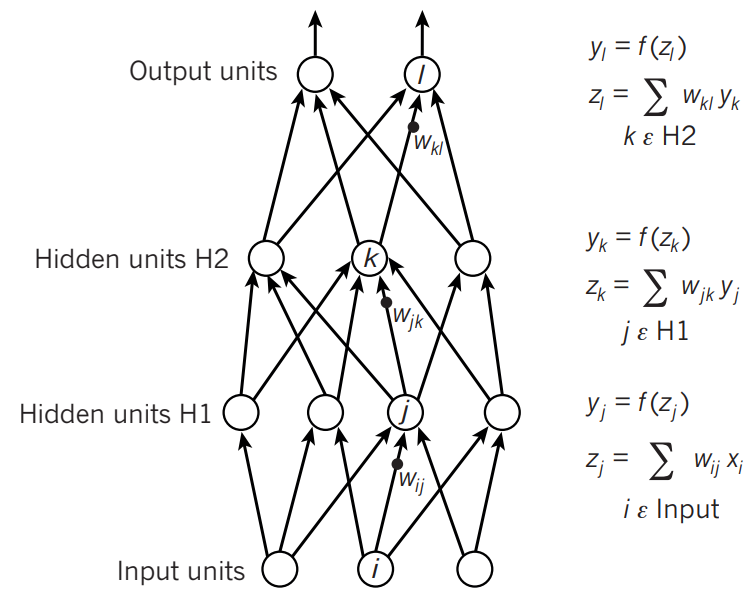
\includegraphics[width=9cm]{nn.png}
	\bicaption[Illustration of Neural Network]
	{多层神经网络示意图}
	{An example of multi-layer neural network. Figure borrowed from \cite{lecun2015deep}}
	\label{fig:nn}
\end{figure}
This paper will be mainly using convolutional neural networks for image recognition. A convolutional layer is different in the mathematical operation, but can feed-forward and back-propagate in the same way. A typical convolutional neural network consists of convolutional layers, pooling layers and fully-connected layers. Fully-connected layer is the same as a single layer neural network. Convolutional layers and pooling layers are illustrated in Fig.~\ref{fig:convolve} and Fig.~\ref{fig:pooling} respectively. 
\begin{figure}[!htp]
	\centering
	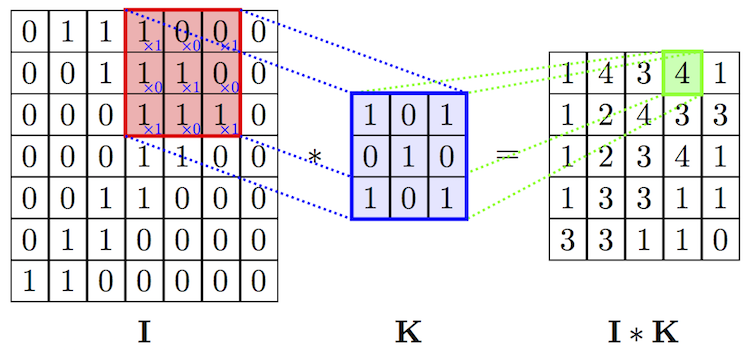
\includegraphics[width=8cm]{convolve.png}
	\bicaption[Illustration of Convolutional Layer]
	{卷积层示意图}
	{Illustration of Convolutional Layer}
	\label{fig:convolve}
\end{figure}
\begin{figure}[!htp]
	\centering
	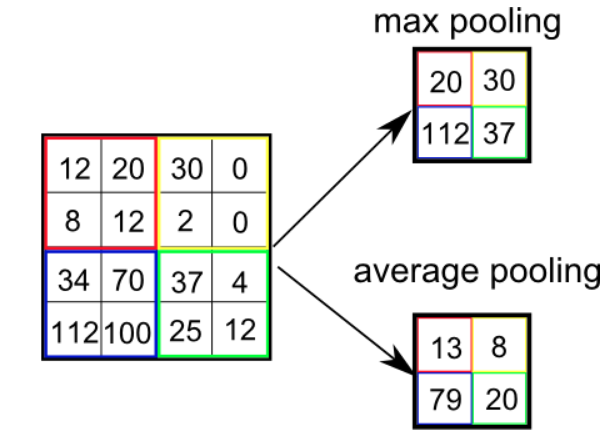
\includegraphics[width=8cm]{pooling.png}
	\bicaption[Illustration of Pooling Layer]
	{池化层示意图}
	{Illustration of Pooling Layer}
	\label{fig:pooling}
\end{figure}

The history and development of deep neural networks, especially for computer vision, has been elaborated in the related work section. In this section, we will introduce several networks in more detail about their architectures, since they are used in the experiments.

\subsection{ResNet}
Deep residual networks\cite{he2016deep}(ResNet) are proposed by Kaiming He in 2015. Before the emergence of deep residual networks, the deepest public network, i.e., the VGGNet, has no more than 40 layers. The introduction of Batch Normalization enabled easier training of deeper networks, but there are only minor improvements in depth. Residual networks completely changed this situation and pushed the barrier of deep networks into more than one hundred layers. 
\begin{figure}[!htp]
	\centering
	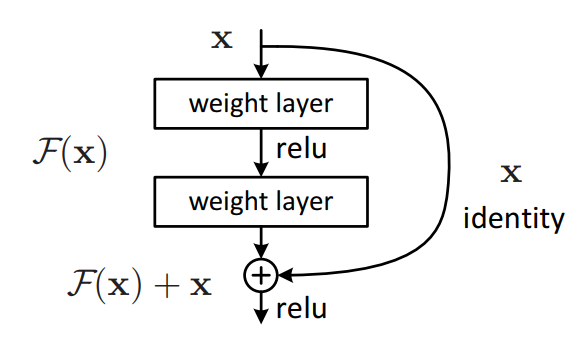
\includegraphics[width=8cm]{resnet.png}
	\bicaption[Illustration of Residual Blocks]
	{残差结构示意图}
	{Illustration of Residual Blocks. Figure borrowed from \cite{he2016deep}.}
	\label{fig:resnet}
\end{figure}

As shown in Fig.~\ref{fig:resnet}, residual networks are based upon residual blocks. In each of the block, a shortcut connection connected the previous layer and the next layer, and adds directly the result. Using this kind of block, one can easily imagine, increasing depth will at least not let the accuracy become worse, because the worst case is to learn an identity mapping. Without the residual connections, the convolutional layer is very hard to learn identity function. Therefore, deeper network become really hard to train. That is the reason why accuracy strangely becomes lower when the network grows deeper. 

There are mainly two views on the most important reason why residual networks are able to learn such deep representations and improve the performance.
\begin{itemize}
	\item The first view is that the identity mappings are the major reason. Since we initialized the network to be near to identity, the accuracy is very unlikely to drop. This reason is also revealed in the paper.
	\item A second view thinks the most important reason is that the residual connections pass the gradients more smoothly, so that the network becomes much easier to learn.
\end{itemize}
There are debates on which of these two views are correct. A paper on Arxiv once claimed that identity mappings are not important because other identity mapping functions are not able to bring about the same good result. Till now, the debate continues, but most experts would like to wait for mathematical proofs regarding deep neural networks, rather than debating and guessing empirically. 

Deep residual networks brought a storm in the field of machine learning. Although it is initially developed for image classification, it is also able to greatly boost the performance of other computer vision tasks such as object detection and segmentation when substituting the base network with deep residual networks in their algorithm. What's more, the same heuristics is quite generic and it is quickly successfully applied to other areas like natural language processing. For example, when people use the same residual connection techniques on Long Term Short Memory model, it also greatly boosted the performance on natural language processing.
\begin{figure}[!htp]
	\centering
	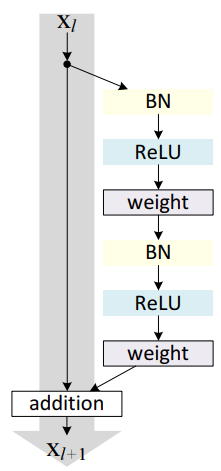
\includegraphics[width=4cm]{resnetv2.png}
	\bicaption[Illustration of Pre-activation Residual Blocks]
	{预激活残差结构示意图}
	{Illustration of Pre-activation Residual Blocks. Figure borrowed from \cite{he2016identity}.}
	\label{fig:resnetv2}
\end{figure}
One year later, the same authors published another paper\cite{he2016identity} and discussed different structures of residual blocks. They improved the residual block of the original paper, and the best residual block is shown in Fig.~\ref{fig:resnetv2}, called the pre-activation structure. Using the better residual block, they are able to train a network much more deeper, up to one thousand two hundred and two layers. They are the first to design a network that operates on more than one thousand layer while also improving accuracy. This version of deep residual network is also called ResNet V2 in literature. 

However, later comments reveal that ResNet V2 actually does not have such significant improvements than ResNet V1. The accuracy difference between them is often very little. Moreover, for some network structures, it would even be better to use ResNet V1. For example, the later network variant ResNext, followed the basic outline of ResNet V1 and achieved state-of-the-art accuracy during the time it was made public.

\subsection{DenseNet}
\begin{figure}[!htp]
	\centering
	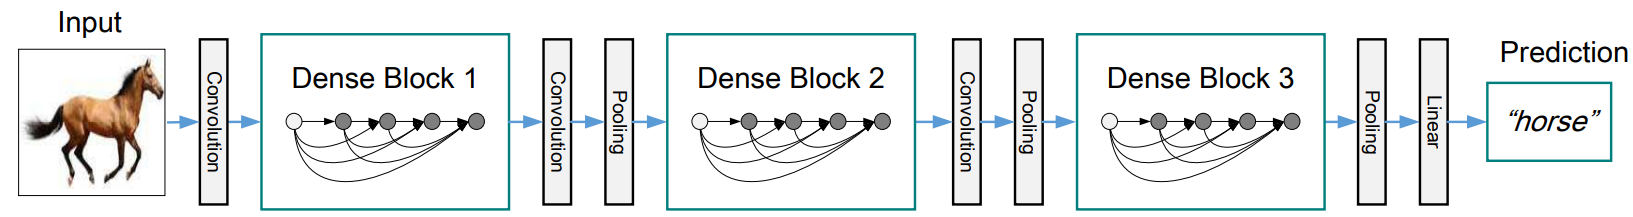
\includegraphics[width=16cm]{densenet.png}
	\bicaption[Illustration of DenseNet]
	{密集链接网络示意图}
	{Illustration of DenseNet. Figure borrowed from \cite{huang2017densely}.}
	\label{fig:densenet}
\end{figure}
Densely Connected Convolutional Networks\cite{huang2017densely} are called DenseNet. A basic block is illustrated in Fig.~\ref{fig:densenet}. It received the CVPR 2016 best paper award, because its novel architecture and further improved the image classification performance of deep residual networks.

To begin with, Densely Connected Convolutional Networks has the following to major difference compared to deep residual networks:
\begin{itemize}
	\item The skip connections has become much denser. They added every possible connection to the current layer. Since it is much denser, the authors name it DenseNet. It is worth noting that the Densely Connected Convolutional Networks is divided into different stages, so the dense connections actually take place only within each stage. If the connections take place on the whole network, the network would be too complicated to calculate or fit in memory. And the feature map size is different, thus restricting the dense connections only in the same stage.
	\item The operation to perform is changed to concatenation rather than summation. This change is quite match to common logic, because with such dense connections, it will become problematic to add all the values from previous layers. By concatenation, one would expect that the feature map dimensions of the later layers to become very large. The authors ameliorate this problem by two means: reduce the natural dimensions of layers so that the number of dimensions is small in the beginning, and add additional layers between stages to map the high dimension feature maps to lower dimensions.
\end{itemize}

Densely Connected Convolutional Networks achieved impressive results on image classification. Besides providing even better flow of gradients to deeper layers, the authors anticipate that by dense connections, the mathematical plane learned by the deep network become more smooth. In this way, the network is easier to find better local optima, and inherently holds some regularization properties.

However, there are also critics that the Densely Connected Convolutional Networks do not perform well when working as a base model when pretrained and used in other tasks like object detection and segmentation. Nowadays, the major view of Densely Connected Convolutional Networks is that its transfer ability is quite weak as a pre-trained feature extractor. A possible reason is that the effective feature map dimensions are so shallow that higher-level general features become very hard to learn. But Densely Connected Convolutional Networks perform well when we try to train a object detection or segmentation base network directly based on the detection or segmentation data, perhaps because of ease of training.

\subsection{ResNeXt}

ResNext is a state-of-the-art convolutional network in 2017\cite{xie2017aggregated}. When combined with Squeeze-and-Excite blocks, it is still the current state-of-the-art network architecture.
\begin{figure}[!htp]
	\centering
	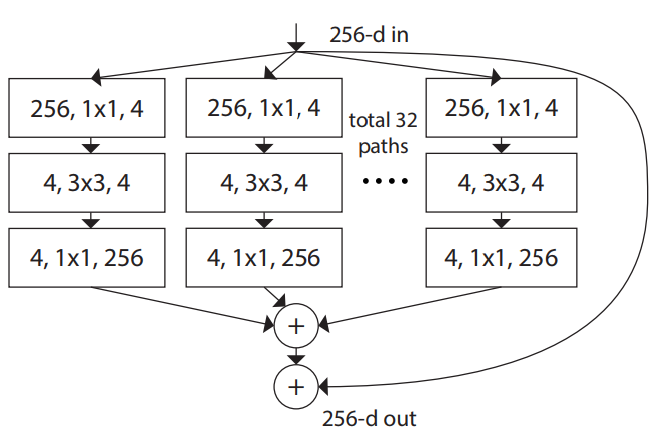
\includegraphics[width=8cm]{resnext.png}
	\bicaption[Illustration of ResNeXt blocks]
	{聚合变换残差网络示意图}
	{Illustration of ResNeXt blocks. Figure borrowed from \cite{xie2017aggregated}.}
	\label{fig:resnext}
\end{figure}
Although stated very complicated in the paper, ResNeXt can be simply explained as ResNet combined with group convolution. A group convolution is illustrated in Fig.~\ref{fig:resnext}.  A normal convolution takes all previous feature map dimensions into calculation for every neuron. But in group convolution, feature map dimensions are divided equally into groups. The convolution layer can also be seen as operates on different groups and finally the results of different groups are concatenated together along the dimension.

Group convolution was first used in AlexNet, in order to fit the network in two GPUs. No earlier work has observed that group convolution is able to boost the network performance. In fact many people have tried it, but the performance might be hard to tune. An important property of group convolutions is that it saves computation and parameters by the group number constant. By making heavy use of group convolution, ResNext is able to become much deeper and wider. In such a way, the network capacity becomes huge.
